\documentclass{article}

% images
\usepackage{graphicx}
\usepackage{caption}
\usepackage{float}

% margins and spacing
\usepackage[a4paper,width=150mm,top=25mm,bottom=25mm]{geometry}
\usepackage{titlesec}
\titlespacing{\section}{0pt}{3em}{1em}

% math and equations
\usepackage{amsmath} 
\numberwithin{equation}{section}

% tables
\usepackage{multirow}

% bold math
\usepackage{bm}

% plots
\usepackage{pgfplots}

% customizing enumerate labels
\usepackage{enumerate} 

% hyperlinks
\usepackage{hyperref}

% units
\usepackage{siunitx}

% highlighting
\usepackage{color}
\usepackage{soul}

\title{\textbf{EW-2 Project 2 Proposal} \\ Theremin}
\author{Krish Pandya \\ krish.pandya@students.iiit.ac.in \\ 2023102026 
        \and 
        Vaibhav Wadhwani \\ vaibhav.wadhwani@students.iiit.ac.in \\ 2023102058}
\date{4th February 2025}

\begin{document}

\maketitle

\section{Project Proposal}
This project proposes the design and construction of a modern Theremin, a touchless electronic musical instrument that merges classic analog circuitry with contemporary design techniques. The instrument will convert subtle human gestures into continuously variable musical tones by utilizing oscillator and amplifier circuits. The primary objectives of the project are as follows:
\begin{enumerate}
    \item To develop reliable oscillator circuits using CMOS logic and analog components that generate controllable waveforms.
    \item To employ the LM386 audio amplifier for clear and effective sound amplification.
    \item To implement a responsive control mechanism that accurately translates hand movements into frequency variations.
    \item To evaluate the system performance in terms of sound quality, responsiveness, and overall stability.
\end{enumerate}
This project not only applies fundamental principles of electronic circuit design but also explores innovative methods of human-machine interaction.

\section{Working Principle of a Theremin}
A Theremin operates using two key principles: capacitance variation and heterodyning. The instrument typically features two antennas; one controls pitch and the other controls volume. The pitch antenna is connected to a high-frequency oscillator. When a performer moves their hand near the antenna, the capacitance in the oscillator circuit changes, altering the frequency slightly. This frequency-modulated signal is then mixed with a fixed reference frequency in a process known as heterodyning, producing an audible beat frequency that changes according to hand movement. The volume antenna, in contrast, modulates the amplitude of the output signal by sensing proximity, allowing for dynamic control of the loudness. Together, these mechanisms allow the performer to manipulate both pitch and volume without physical contact, creating a unique and expressive instrument.


\section{Project Requirements}

\begin{figure}[H]
    % \centering
    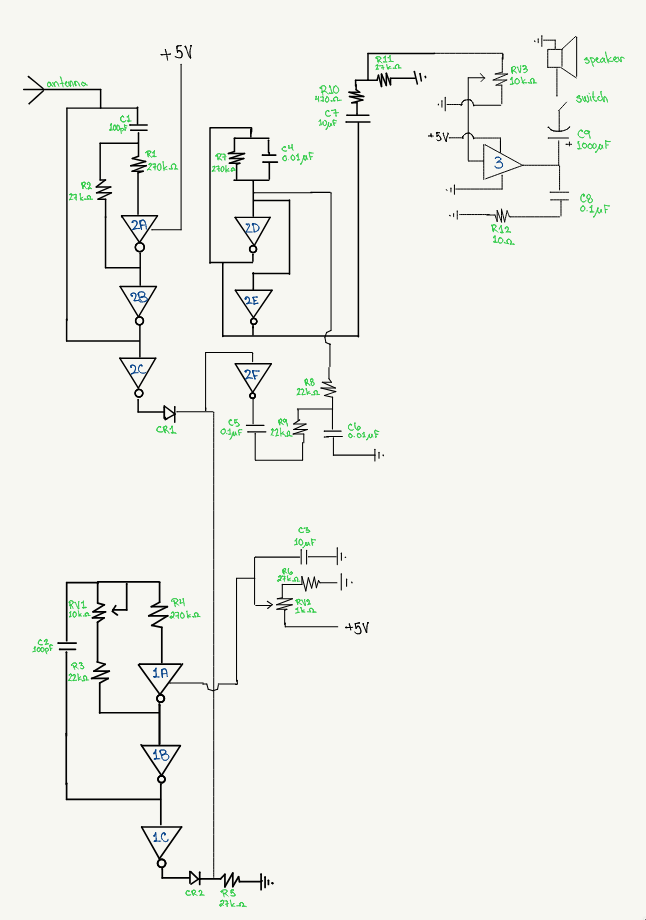
\includegraphics[width=0.5\textwidth]{theremin_circuit.png}
    \caption{Theremin Schematic}
    \label{fig:theremin}
\end{figure}

The following list details the critical components required for the project:

\subsection*{Integrated Circuits}
\begin{itemize}
    \item \textbf{CMOS CD4069UBE hex inverter (3 units):} Used for signal inversion and waveform generation in the oscillator sections.
    \item \textbf{LM386 audio amplifier (1 unit):} Amplifies the generated audio signal to drive a speaker efficiently.
\end{itemize}

\subsection*{Resistors}
\begin{itemize}
    \item 10 Ohm resistor (1 unit)
    \item 27 kOhm resistor (5 units)
    \item 22 kOhm resistor (3 units)
    \item 270 kOhm resistor (4 units)
    \item 470 kOhm resistor (1 unit)
    \item 1 kOhm variable resistor (1 unit)
    \item 10 kOhm variable resistor (2 units)
\end{itemize}

\subsection*{Capacitors}
\begin{itemize}
    \item 100 pF capacitor (3 units)
    \item 0.01 µF capacitor (2 units)
    \item 0.1 µF capacitor (2 units)
    \item 10 µF capacitor (2 units)
    \item 1000 µF capacitor (1 unit)
    \item 1 nF variable capacitor (1 unit)
\end{itemize}

\subsection*{Other Electronics}
\begin{itemize}
    \item \textbf{Diodes (2 units):} Provide circuit protection and assist in signal rectification.
    \item \textbf{Slide Switch (e.g., SS22D18) (1 unit):} Facilitates power control or mode selection within the circuit.
    \item \textbf{Speaker (e.g., 0.2 W, 8 Ohm breadboard mount speaker) (1 unit):} Outputs the amplified audio signal.
    \item \textbf{5V Power Supply (1 or 2 units):} Ensures a stable operating voltage for the entire circuit.
\end{itemize}

\section{Conclusion}
The proposed Theremin project ties together essential electronic principles with a musical application. By leveraging both standard and variable components, the instrument will respond to user gestures, offering a unique interface and auditory experience.

\end{document}